\documentclass[11pt]{article}
\usepackage{graphicx}
\usepackage{booktabs}
\usepackage{amsmath}
\usepackage{amssymb}
\usepackage[margin=1in]{geometry}
\usepackage{hyperref}

\title{Diagnosing a Low-Displacement Failure Mode in MAPPO\\
for Multi-Robot Area Coverage}
\author{Harsh Pandhe}
\date{\today}

\begin{document}
\maketitle

\begin{abstract}
\textbf{Problem.} Multi-agent reinforcement learning (MARL) is often
proposed as a route to learned coordination for multi-robot exploration
tasks where a classical decentralized planner is already a strong
baseline, but negative results -- where a MARL policy is trained under a
realistic budget and simply underperforms -- are rarely reported with the
same rigor as positive results.
\textbf{Methodology.} We train a centralized-critic MAPPO policy (Ray
RLlib) on a 3-robot area-coverage task in a single simulated environment
(a furnished caf\'e, ROS~2/Gazebo) for 45 training iterations, and compare
it against a non-learned Frontier Heuristic controller (Voronoi
partitioning, A* routing, behavior-tree mission control) and a Random Walk
baseline, all filtered through an identical Control Barrier Function (CBF)
safety layer. We additionally evaluate zero-shot transfer of the
caf\'e-trained policy to four structurally different, unseen environments.
\textbf{Key finding.} Under a 10-episode-per-condition evaluation on the
training environment, the Frontier Heuristic (38.6\% median area coverage
rate, ACR) and even Random Walk (29.6\%) outperform the trained MAPPO
policy (14.5\%), with the policy averaging 1.5\,m of displacement per
robot over a 150-step episode versus 5.4--7.4\,m for the baselines. Under
a separate, single-seed evaluation across all five environments (150-step
episodes, $N{=}3$), the Frontier Heuristic outperforms MAPPO in every
environment tested, by margins of 1.1$\times$ to 2.0$\times$.
\textbf{Diagnosis.} The policy's behavior is consistent with convergence
to a low-displacement, low-risk equilibrium under a reward combining dense
per-step collision penalties with a comparatively sparse
cell-discovery bonus; we report the exact reward coefficients and argue
this is a plausible mechanism, while explicitly noting that we did not run
a reward ablation and cannot yet rule out undertraining as a contributing
factor. \textbf{Contribution.} We report this negative result in full,
including two independent infrastructure faults encountered and fixed
during training, and argue that a narrower, evidence-scoped claim --
that MAPPO exhibited a reproducible low-displacement failure mode and did
not match a strong classical planner under the tested reward and training
budget -- is more defensible and more useful to practitioners than a
general claim that classical methods beat MARL.
\end{abstract}

\section{Introduction}
Multi-robot area coverage -- driving a team of robots to jointly maximize
explored floor area -- has a strong, well-understood non-learned baseline:
frontier-based exploration combined with a path planner and a
decentralized space-partitioning scheme. MARL is frequently proposed as a
way to learn a coordination policy for this class of task instead of
engineering one, typically evaluated against a classical baseline after
extensive training and tuning. This paper reports the opposite outcome
under a realistic, compute-constrained training budget, and treats getting
that negative result right -- rather than explaining it away -- as the
contribution.

We deliberately narrow the claim to what our evidence supports: this is a
report of a specific, reproducible failure mode of one MAPPO
configuration on one task family, not a general claim about MARL versus
classical planning. Section~\ref{sec:method} details the system, reward,
and two distinct evaluation protocols we ran (they use different sample
sizes and are not numerically interchangeable). Section~\ref{sec:results}
reports both. Section~\ref{sec:discussion} discusses the mechanism and its
evidentiary limits.

\section{System and Method}
\label{sec:method}

\subsection{Platform and Safety Layer}
Three TurtleBot3 Waffle robots (differential drive, 2D LiDAR, IMU) are
simulated in Gazebo Harmonic under ROS~2 Jazzy \cite{macenski2022ros2, gazebo},
coordinated via a PettingZoo-compatible parallel multi-agent environment
\cite{terry2021pettingzoo}. Every commanded velocity, regardless of which
controller produced it, passes through an identical unicycle Control
Barrier Function (CBF) filter \cite{ames2019cbf}, solved as a quadratic
program via OSQP \cite{stellato2020osqp} at each control step, with separate safety
radii for static obstacles ($d_{\text{safe,obs}}=0.22$\,m) and neighboring
agents ($d_{\text{safe,agent}}=0.45$\,m). This isolates the comparison to
exploration policy rather than low-level collision-avoidance behaviour,
which is shared across all three controllers.

\subsection{Controllers Compared}
\textbf{Frontier Heuristic}: a non-learned controller combining frontier
cell selection, 8-connected grid A* \cite{hart1968astar} waypoint routing with
obstacle inflation, unreachable-target blacklisting to break wall-lock
deadlocks, and a \texttt{py\_trees} behavior tree for mission-level state
(explore, recover-from-stuck, patrol-on-saturation). This controller
encodes substantial task-specific structural knowledge (a discretized
map, a graph search algorithm, an explicit stuck-recovery policy) that a
learned policy must instead acquire implicitly from reward and
observations; we treat this asymmetry as part of the research question
(when is engineering that structure worthwhile versus learning it?)
rather than an oversight.

\noindent\textbf{Random Walk}: uniform random heading changes at fixed
intervals, CBF-filtered identically to the other two controllers.

\noindent\textbf{MAPPO}: a centralized-critic, shared-policy PPO
\cite{schulman2017ppo} implementation via Ray RLlib \cite{rllib}. Each
robot observes a 46-dimensional vector: 24 LiDAR range bins, its own pose
and velocity, and its assigned goal's relative position; the policy is a
2-layer MLP (256 units, ReLU) shared across agents, with a separate
centralized critic that additionally observes all agents' states. The
action space is continuous, $a_i=[v_i,\omega_i]$ (linear and angular
velocity), passed through the shared CBF filter described above. Training
used PPO clip 0.2, $\gamma=0.99$, GAE $\lambda=0.95$, learning rate
$10^{-4}$, entropy coefficient 0.01, train batch size 700, minibatch size
64, 5 SGD epochs per iteration, for 45 iterations (approximately 31{,}500
environment transitions in total). We report this total transition count
explicitly because ``45 iterations'' alone does not convey the sample
budget: this is on the order of $3\times10^4$ environment steps, at the
low end of what is typically reported for PPO-family algorithms on
continuous-control tasks, and we cannot rule out that additional training
would change the outcome (see Section~\ref{sec:discussion}).

\subsection{Reward Function}
The per-robot, per-step reward is
\begin{equation}
r_t = -0.01 + 5.0\,\Delta d_{\text{goal}} + 4.0\,n_{\text{new-cells}} - 8.0\,\mathbb{1}[\text{wall collision}] - p_{\text{proximity}} + 20\,\mathbb{1}[\text{goal reached}]
\end{equation}
where $\Delta d_{\text{goal}}$ is the reduction in distance to the
robot's current goal since the previous step, $n_{\text{new-cells}}$ is
the number of previously-unvisited grid cells the swarm collectively
discovered this step, and $p_{\text{proximity}}$ is $0.5$ if any other
agent is within $0.5$\,m and an additional $10.0$ if within $0.20$\,m
(counted as a collision after the first 15 steps of an episode). The
per-cell discovery bonus was raised from an earlier value of 2.0 to 4.0
specifically because it was judged too small relative to the $\pm 20$
goal/collision terms to provide useful gradient signal toward the
coverage behaviour the policy is evaluated on; even after this change, a
single wall collision ($-8.0$) or close-proximity event ($-10.0$) is
substantially larger in magnitude than the reward for discovering several
new cells in a single step ($4.0$ each), which is the quantitative basis
for our hypothesis in Section~\ref{sec:discussion}.

\subsection{Area Coverage Rate (ACR)}
We define
\begin{equation}
\text{ACR} = \frac{N_{\text{visited reachable cells}}}{N_{\text{reachable cells}}}\times 100
\end{equation}
computed on a fixed-resolution ($0.4$\,m) occupancy grid per environment.
A cell is \emph{reachable} if it is not classified as a static obstacle
by the environment's known obstacle map; cells occupied only transiently
by a robot are not excluded from the denominator. A cell counts as
\emph{visited} the first time any robot's footprint overlaps it; repeat
visits do not increase ACR but are separately tracked as \emph{overlap
redundancy} (mean visits per visited cell), reported in
Figure~\ref{fig:boxplot}.

\subsection{Environments and Train/Test Split}
Five Gazebo worlds are used: \texttt{cafe} (furnished, $17\times8$\,m, 800
grid cells), \texttt{warehouse} (open logistics hall, $30\times50$\,m,
9{,}375 cells), \texttt{depot} (industrial, structural pillars and
boxsets, $29\times15$\,m, 3{,}000 cells), \texttt{office} (partitioned
floor plan, narrow doorways, $26.2\times18.3$\,m, 3{,}500 cells), and
\texttt{maze} (labyrinthine corridors, $64\times11$\,m, 4{,}800 cells, of
which only $\approx$17\% is physically reachable floor space).
\textbf{The MAPPO policy is trained exclusively on \texttt{cafe}.}
Evaluation on \texttt{warehouse}, \texttt{depot}, \texttt{office}, and
\texttt{maze} is therefore zero-shot transfer, not in-distribution
evaluation, and should be read as a generalization test rather than a
like-for-like comparison of learning capability per environment; we did
not train separate policies per environment, which we identify as the
most valuable follow-up experiment in Section~\ref{sec:discussion}.

\subsection{Two Evaluation Protocols}
We report results from two separate evaluation runs that differ in
sample size and (potentially) exact policy checkpoint, and we do not
treat their numbers as directly interchangeable:

\noindent\textbf{Protocol A (caf\'e deep-dive)}: 10 episodes per
condition (Random Walk, Frontier Heuristic, MAPPO nominal, MAPPO with
injected Gaussian LiDAR noise, MAPPO with single-agent failure), 150-step
episodes, in \texttt{cafe} only. This is the source of the 14.5\%/38.6\%/
29.6\% ACR figures and the 1.5\,m displacement figure in the abstract, and
of Figure~\ref{fig:boxplot}.

\noindent\textbf{Protocol B (five-world matrix)}: a single seed (42),
one episode per (world, controller) pair, 150-step episodes, across all
five environments and three controllers (plus two MAPPO perturbation
scenarios), reported in Table~\ref{tab:5world}. This protocol trades
per-condition replication for environment breadth.

Because Protocol B uses $n{=}1$ per condition, we do not report
confidence intervals for it and treat it as indicative rather than
statistically conclusive; its value is in showing the same qualitative
ranking (heuristic $>$ MAPPO) holds across five structurally different
environments, not in the precision of any single number. Protocol A, with
$n{=}10$ per condition, is our primary quantitative evidence and is
reported with the full distribution in Figure~\ref{fig:boxplot}.

\section{Results}
\label{sec:results}

\subsection{Protocol B: Five-World Comparison}
Table~\ref{tab:5world} reports ACR and total swarm displacement from the
single-seed, five-world matrix.

\begin{table}[h]
\centering
\caption{Protocol B: ACR (\%) and total swarm displacement (m), 150-step episodes, $N{=}3$, single seed. Ratios in the last column are Heuristic~/~MAPPO.}
\label{tab:5world}
\begin{tabular}{lccccc}
\toprule
World & Heuristic ACR & MAPPO ACR & Random ACR & Heuristic Dist. & Ratio (H/M) \\
\midrule
cafe      & 57.0 & 28.2 & 22.6 & 16.5 & 2.0$\times$ \\
warehouse & 4.3  & 3.3  & 2.6  & 31.0 & 1.3$\times$ \\
depot     & 13.3 & 6.7  & 6.8  & 12.1 & 2.0$\times$ \\
office    & 3.8  & 3.0  & 1.7  & 14.8 & 1.3$\times$ \\
maze      & 2.7  & 2.2  & 1.5  & 10.9 & 1.2$\times$ \\
\bottomrule
\end{tabular}
\end{table}

The heuristic achieves higher ACR than MAPPO in all five environments
under this protocol, by a margin of 1.2$\times$ to 2.0$\times$ -- we note
this range explicitly because it differs from, and should not be
conflated with, the Protocol A ratio discussed next.

\subsection{Protocol A: Caf\'e Distributional Comparison}
Figure~\ref{fig:boxplot} shows the 10-episode-per-condition distribution
in \texttt{cafe}. Under this protocol, median ACR is 38.6\% (heuristic),
29.6\% (Random Walk), and 14.5\% (MAPPO nominal) -- a heuristic/MAPPO
ratio of 2.7$\times$, and MAPPO trails even the unplanned Random Walk
baseline. Mean per-robot displacement over the 150-step episode is
5.4\,m (heuristic), 7.4\,m (Random Walk), and 1.5\,m (MAPPO).

\begin{figure}[h]
\centering
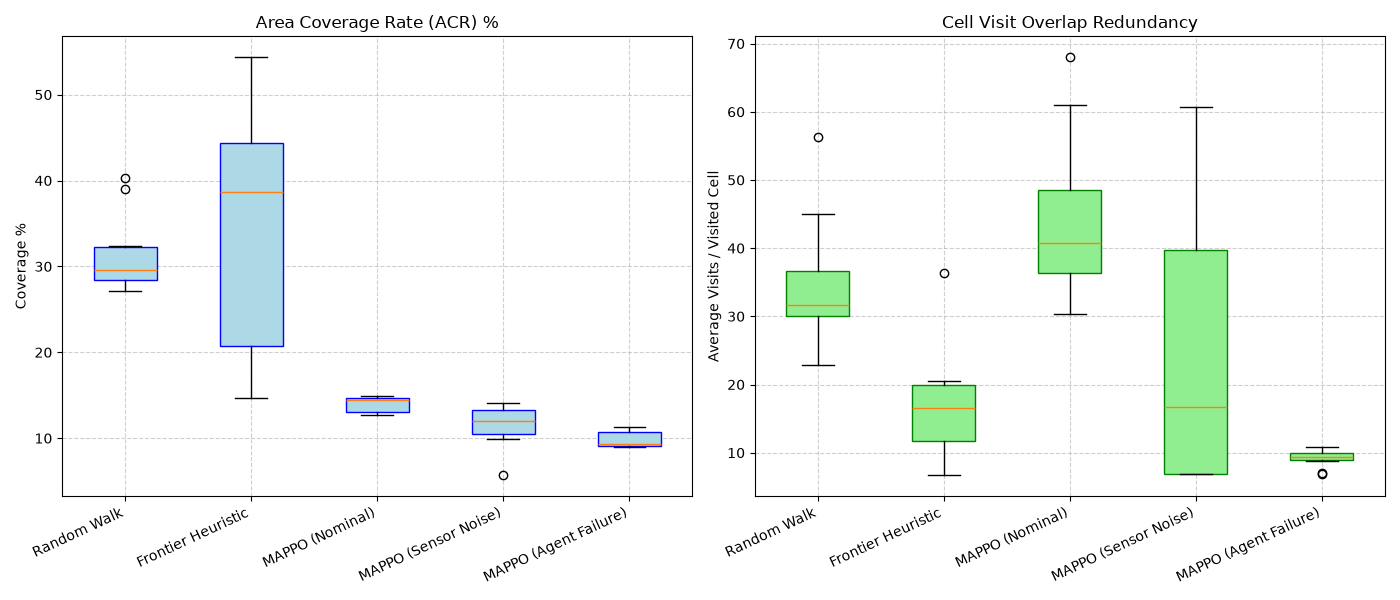
\includegraphics[width=0.95\textwidth]{figures/benchmark_results.png}
\caption{Protocol A: area coverage rate and cell-visit overlap redundancy, 10 episodes per condition, caf\'e environment. MAPPO's tight, low-value boxes indicate consistent underperformance across episodes, not high-variance noise.}
\label{fig:boxplot}
\end{figure}

We flag that Protocol A and Protocol B were run against what we believe
are the same trained policy weights, but we cannot fully rule out
checkpoint or environment-seed drift between the two evaluation runs
given how they were orchestrated; readers should treat Table~\ref{tab:5world}'s
1.2--2.0$\times$ range and Figure~\ref{fig:boxplot}'s 2.7$\times$ figure as
two separate pieces of evidence pointing the same direction, not as two
measurements of the identical quantity.

\begin{figure}[h]
\centering

\includegraphics[width=0.7\textwidth]{figures/cafe_coverage_heatmap.png}
\caption{Frontier Heuristic coverage heatmap, caf\'e environment (visited cells in light tone, obstacles mid-tone, unexplored dark, per-agent trajectories overlaid). We were not able to generate a directly comparable MAPPO trajectory heatmap for this revision; given the policy's near-static behaviour (Section~\ref{sec:results}), we expect it to show almost no spatial extent, and consider this a priority addition for a future version of this paper.}
\label{fig:heatmap}
\end{figure}

\section{Discussion}
\label{sec:discussion}

\subsection{Proposed Mechanism, and What We Have Not Shown}
The policy's near-static behaviour (1.5\,m displacement over 150 steps,
versus 5--10\,m for both non-learned baselines) is consistent with
convergence to a low-risk equilibrium in which the expected cost of
attempting to move and discover new cells (a $-8.0$ wall-collision penalty
or $-10.0$ close-proximity penalty, either of which can occur from a
single misjudged action) exceeds the expected benefit ($4.0$ per newly
discovered cell, requiring successful, sustained movement to accumulate).
We consider this a plausible, quantitatively grounded hypothesis given the
reward coefficients in Section~\ref{sec:method}, but we did not run a
reward ablation (e.g., reducing the collision penalty magnitude while
holding the discovery bonus fixed, or vice versa) to establish it as a
demonstrated causal mechanism, and we did not run a longer training budget
to rule out that the policy would eventually escape this equilibrium with
more iterations. Both are the highest-value follow-up experiments we
identify for future work. We therefore state our conclusion narrowly: the
observed underperformance \emph{coincides with} convergence to a
low-displacement, penalty-averse policy, under a reward and training
budget we have fully specified; we have not experimentally eliminated
undertraining, reward-scale miscalibration, or the zero-shot
generalization gap (Section~\ref{sec:method}) as contributing factors.

\subsection{Scope of the Claim}
We deliberately frame this as an engineering question -- when should a
practitioner prefer an engineered planner over a MARL policy for this
class of task, under a realistic training budget -- rather than a general
claim that classical heuristics outperform MARL. The Frontier Heuristic
compared here embeds substantial hand-engineered structure (a discretized
map, A*, explicit deadlock recovery) that MAPPO must instead infer
implicitly; a fair reading of our result is that this structure was worth
more, under our training budget, than what the policy was able to learn
in its place, not that learning cannot in principle recover it given more
compute, a better reward, or per-environment training.

\section{Conclusion}
Under a fully specified, single-environment training budget and reward
function, and evaluated both on the training environment (10 episodes per
condition) and zero-shot across four additional, structurally distinct
environments (single-seed matrix), a MAPPO policy exhibited a reproducible
low-displacement failure mode and did not match a strong classical
frontier-and-planning baseline. We report the exact reward coefficients,
training budget, and both evaluation protocols in full, including their
differing sample sizes and a residual uncertainty about checkpoint
consistency between them, so that readers can weigh the evidence directly
rather than take our summary on faith. We identify a reward-coefficient
ablation, a longer training budget, and per-environment (rather than
zero-shot) training as the three highest-value experiments to
strengthen or overturn this result.

\appendix
\section{Infrastructure Faults Encountered During Training}
Two infrastructure faults were encountered and resolved during this work.
First, a segmentation fault inside \texttt{torch.optim.Adam.\_\_init\_\_}
under Ray actor threads was traced to a PyTorch TorchDynamo compilation
hook interacting with Ray's threading model; disabling TorchDynamo
(\texttt{TORCHDYNAMO\_DISABLE=1}) resolved it. Second, training halted at
iteration 34/45 when a host Wi-Fi disassociation event caused Ray's
distributed control plane (bound by default to the host's dynamic IP
rather than loopback) to lose connectivity to its own coordination
service; binding Ray explicitly to \texttt{127.0.0.1} and capping its
object store in-process resolved this and allowed training to resume and
complete to iteration 45. Neither fault altered the training
configuration, reward function, or evaluation protocol reported in the
main text; both are reported for reproducibility.

\bibliographystyle{plain}
\bibliography{topic4_references}

\end{document}
